%documentMetadata{}
\documentclass[a4paper,12pt]{article}

%\usepackage[italian]{babel}
\usepackage{pgfplots}
\usepackage{amsmath}
\usepackage{float}
\usepackage{graphicx} %for the scheme
\usepackage{array}
\usepackage[margin=1in]{geometry}
\pgfplotsset{width=10cm,compat=1.9}

\begin{document}

\parskip=10pt plus 1pt
\parindent=0pt

\begin{center}
    University of Milan

\par{\Large{Optics, Electronics, and Modern Physics Laboratory}}  

December 20, 2024 

Group ME6
\par


\end{center}
\par\noindent\rule{\textwidth}{0.4pt}

\begin{abstract}
    \begin{center}
    \par{\large{Lab report: Measuring the charge-to-mass ratio of the electron}}

    Text here
    
    \end{center}
\end{abstract}

\par\noindent\rule{\textwidth}{0.4pt}


%Scopo e modalità (in breve) 
%Descrivere sinteticamente ciò che ci si propone di fare 
%nell'esperimento, ossia cosa si vuole misurare, verificare, provare… Cosa 
%si dovrà misurare? Con che strumento? Potete inserire foto o schemi.
\section{Objectives}
%\documentclass{article}
%\usepackage{amsmath}
%\usepackage{graphicx}
%\usepackage{tikz}

%\begin{document}

%\section*{Objectives}

The purpose of this experiment is to determine the charge-to-mass ratio $e/m$ for an electron by observing and analyzing the behavior of electrons accelerated under controlled electric and magnetic fields. Electrons are emitted from an heated filament by thermionic emission and subsequently accelerated by a known potential difference $\Delta V$. This energy provides the electrons with a specific kinetic energy, allowing them to enter the magnetic field generated by a pair of Helmholtz coils where a current intensity $I$ flows and generate an uniform magnetic field $B_z$. 

Within this magnetic field, electrons are subjected to the Lorentz force, which causes them to follow a circular trajectory due to the perpendicular orientation of their velocity relative to the field $B_z$. The radius of this trajectory is directly influenced by the balance between the centripetal force and the magnetic force acting on the electrons. 
By systematically varying $\Delta V$ and the current $I$ in the Helmholtz coils, and measuring the electron's trajectory radius $R$, is possible to calculate the $e/m$ ratio from macroscopic variables. 
A mirror behind the setup reduces parallax errors when measuring the electron beam's diameter. 
Measurements are performed in multiple orientations to assess the effect of Earth’s horizontal magnetic field component on the electron trajectory. The setup includes configurations in which the magnetic field of the coils is first orthogonal, then parallel, and finally antiparallel to Earth’s magnetic field.

Moreover, this experiment measures the horizontal component of Earth’s magnetic field by observing deflections of a magnetic needle on which a uniform magnetic field is applied.
%This measurement helps account for Earth’s magnetic influence, enhancing the accuracy of electron dynamics analysis in combined electric and magnetic fields. 

%Errors are minimized by adjusting the setup's orientation and correcting Earth’s magnetic field measurements with a magnetic needle. Adjusting voltage and current stabilizes the beam's path diameter, improving measurement consistency.

This experiment effectively determines the electron’s charge-to-mass ratio by linking electric and magnetic measurements to calculate its circular motion under controlled conditions.

\begin{figure}[h!]
    \centering
    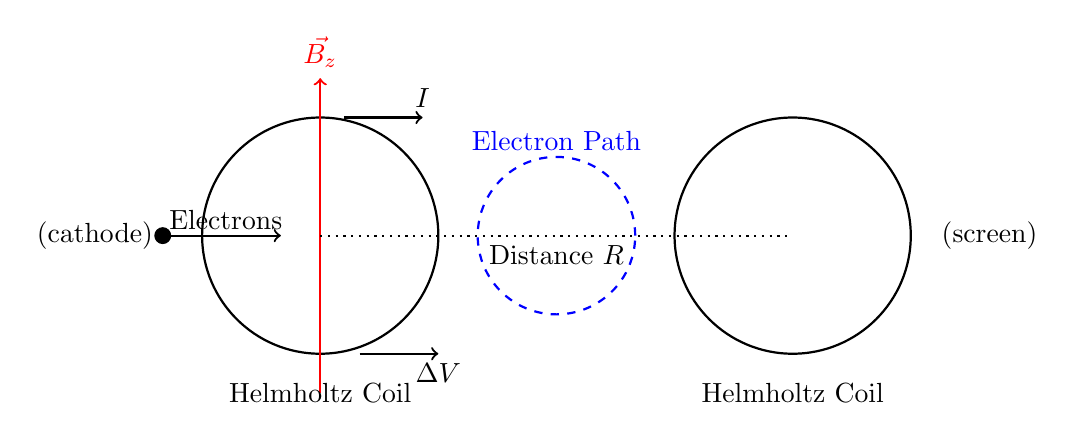
\begin{tikzpicture}
        % Helmholtz coils
        \draw[thick] (-3,0) circle (1.5cm);
        \draw[thick] (3,0) circle (1.5cm);

        % Electron path
        \draw[blue, thick, dashed] (0,0) circle (1cm);
        \node[blue] at (0,1.2) {Electron Path};

        % Electrons/cathode
        \draw[fill=black] (-5,0) circle (0.1cm) node[left] {(cathode)};
        \draw[->, thick] (-5,0) -- (-3.5,0);
        \node at (-4.2,0.2) {Electrons};

        % Magnetic field 
        \draw[->, red, thick] (-3,-2) -- (-3,2) node[above] {$\vec{B_z}$};
        %\node[red] at (-2.7,1.8) {Magnetic Field};

        % Coils (Names)
        \node at (-3, -2) {Helmholtz Coil};
        \node at (3, -2) {Helmholtz Coil};

        %screen
        
        \node at (5.5,0) {(screen)};

        % Connection
        \draw[thick, dotted] (-3,0) -- (3,0) node[midway, below] {Distance $R$};
        

        % V and I
        \draw[->, thick] (-2.7,1.5) -- (-1.7,1.5) node[above] {$I$};
        \draw[->, thick] (-2.5, -1.5) -- (-1.5, -1.5) node[below] {$\Delta V$};

     \end{tikzpicture}
     \caption{Scheme of the Experimental Setup}
    \label{fig:setup}
    \end{figure}

%\end{document}


%Raccolta dati misurati sotto forma di tabella ordinata
%Presentare non solo i dati elaborati ma anche quelli grezzi
%(questi ultimi, eventualmente, in appendice).
%Presentare eventuali grafici con gli assi correttamente definiti (unità di 
%misura, cifre significative, identificativo assi).

\section{Procedure}

%Raccolta dati misurati sotto forma di tabella ordinata
%Presentare non solo i dati elaborati ma anche quelli grezzi
%(questi ultimi, eventualmente, in appendice).
%Presentare eventuali grafici con gli assi correttamente definiti (unità di 
%misura, cifre significative, identificativo assi).


%Sample: Table
%\begin{table}[!htbp]
%    {\par\centering
%    \begin{tabular}{ccccc}
%        \hline
%        Misura & $M \text{ (g)}$ & $\sigma_{M} \text{ (g)}$ & $L \text{ (cm)}$ & $\sigma_{L} \text{ (cm)}$ \\
%        \hline
%        1   &   324.2&   0.1 &   79.5    &   0.1\\
%        2   &   333.7&   0.1 &   79.6    &   0.1\\
%        3   &   344.1&   0.1 &   79.7    &   0.1\\
%        4   &   363.7&   0.1 &   80.0    &   0.1\\
%        5   &   383.4&   0.1 &   80.1    &   0.1\\
%        \hline
%    \end{tabular}
%    \par}
%    \caption{Lunghezza della corda in funzione delle masse appese}
%\end{table}


%Sample: Multiline values
%\begin{align*}
%    &M_{tot} = (20.6 \pm 0.1) \ \text{g} \\
%    &m_{g} = (3.2 \pm 0.1) \ \text{g} \\
%    &L_{r,tot} (77.5 \pm 0.1) \ \text{cm} \\
%    &L_{r} = (75.8 \pm 0.1) \ \text{cm} \\
%\end{align*}

%Sample: Single line value
%\[
%    L_{0}=(78.8 \pm 0.1) \ \text{cm}
%\]


%Sample: Chart
%\begin{center}
%\begin{tikzpicture}
%    \begin{axis}[
%        title=Determinazione costante elastica,
%        xlabel=$L \text{ (m)}$,
%        ylabel=$M_{s} \text{ (kg)}$,
%        minor y tick num=1,
%        minor x tick num=1,
%        x tick label style={
%            /pgf/number format/.cd,
%            fixed,
%            fixed zerofill,
%            precision=3,
%            /tikz/.cd
%        }
%    ]
%        \addplot[color=blue, domain=0.794:0.802]{x*9.079-6.893};
%        \addplot+[scatter, only marks, mark=o, error bars/.cd, y dir=both,y explicit, x dir=both, x explicit, error %mark=-]
%            coordinates {
%                (0.7950,0.3242)   +-  (0.001,0.0001)
%                (0.7960,0.3337)   +-  (0.001,0.0001)
%                (0.7970,0.3441)  +-  (0.001,0.0001)
%                (0.8000,0.3637)  +-  (0.001,0.0001)
%                (0.8010,0.3834)  +-  (0.001,0.0001)
%        };
%    \end{axis}
%\end{tikzpicture}
%\end{center}

%Stima degli errori delle grandezze misurate (giustificare il metodo scelto)
%Valore finale della grandezza da determinare ed incertezza
%Ricordarsi di dare i valori con i rispettive errori e attenzione alle cifre significative! 
\section{Data Analysis}
%Stima degli errori delle grandezze misurate (giustificare il metodo scelto)
%Valore finale della grandezza da determinare ed incertezza
%Ricordarsi di dare i valori con i rispettive errori e attenzione alle cifre significative!

%Sample: Table
%\begin{table}[!htbp]
%    {\par\centering
%    \begin{tabular}{ccccc}
%        \hline
%        Misura & $M \text{ (g)}$ & $\sigma_{M} \text{ (g)}$ & $L \text{ (cm)}$ & $\sigma_{L} \text{ (cm)}$ \\
%        \hline
%        1   &   324.2&   0.1 &   79.5    &   0.1\\
%        2   &   333.7&   0.1 &   79.6    &   0.1\\
%        3   &   344.1&   0.1 &   79.7    &   0.1\\
%        4   &   363.7&   0.1 &   80.0    &   0.1\\
%        5   &   383.4&   0.1 &   80.1    &   0.1\\
%        \hline
%    \end{tabular}
%    \par}
%    \caption{Lunghezza della corda in funzione delle masse appese}
%\end{table}


%Sample: Multiline values
%\begin{align*}
%    &M_{tot} = (20.6 \pm 0.1) \ \text{g} \\
%    &m_{g} = (3.2 \pm 0.1) \ \text{g} \\
%    &L_{r,tot} (77.5 \pm 0.1) \ \text{cm} \\
%    &L_{r} = (75.8 \pm 0.1) \ \text{cm} \\
%\end{align*}

%Sample: Single line value
%\[
%    L_{0}=(78.8 \pm 0.1) \ \text{cm}
%\]


%Sample: Chart
%\begin{center}
%\begin{tikzpicture}
%    \begin{axis}[
%        title=Determinazione costante elastica,
%        xlabel=$L \text{ (m)}$,
%        ylabel=$M_{s} \text{ (kg)}$,
%        minor y tick num=1,
%        minor x tick num=1,
%        x tick label style={
%            /pgf/number format/.cd,
%            fixed,
%            fixed zerofill,
%            precision=3,
%            /tikz/.cd
%        }
%    ]
%        \addplot[color=blue, domain=0.794:0.802]{x*9.079-6.893};
%        \addplot+[scatter, only marks, mark=o, error bars/.cd, y dir=both,y explicit, x dir=both, x explicit, error %mark=-]
%            coordinates {
%                (0.7950,0.3242)   +-  (0.001,0.0001)
%                (0.7960,0.3337)   +-  (0.001,0.0001)
%                (0.7970,0.3441)  +-  (0.001,0.0001)
%                (0.8000,0.3637)  +-  (0.001,0.0001)
%                (0.8010,0.3834)  +-  (0.001,0.0001)
%        };
%    \end{axis}
%\end{tikzpicture}
%\end{center}

\numberwithin{equation}{section}
\numberwithin{table}{section}
\numberwithin{figure}{section}
\subsection{Charge to mass ratio of the electron}
%The coil magnetic field is generated at its centre, as such, 
We found the radius of the coil as the sum of the distance between their outer parts $x_o$ , and their inner distance $x_i$ all divided by 2. We took three measures  and use their arithmetic mean as the final value $x_f=(15,536\pm 0,015)$ cm. Their values, in centimetres, are shown below:

\begin{table}[h!]
    \centering
        \begin{tabular}{|c|c|c|}
            \hline
            \textbf{$X_o$} & \textbf{$X_i$} & \textbf{$X_r$} \\
            \hline
            17,740 & 13,260 & 15,500 \\
            \hline
            17,786 & 13,342 & 15,564 \\
            \hline
            17,780 & 13,310 & 15,545 \\
            \hline
        \end{tabular} 
\end{table}
where $x_r$ is the radius of the coil.  
We took the resolution of the nonius ($\pm 0,001$ cm) as the uncertainty on our measures; the one on the mean was calculated as the standard error of the mean:
\begin{equation*}
    \sigma_{x_f}=\frac{\sigma}{\sqrt{n}}
\end{equation*}
where $\sigma$ is the standard deviation and n the number of measures.
We measured the diameter of the deflected beam of electrons with the same nonius, we took two measures for each case. The values for all configurations are shown in the tables below:
\begin{table}[H]
    \centering
    \begin{tabular}{ccc}
        % Prima tabella
        \begin{tabular}{|c|c|c|}
            \hline
            \multicolumn{3}{|c|}{\textbf{Orthogonal}} \\
            \hline
            \textbf{$D_1$} & \textbf{$D_2$} & Semisum \\
            \hline
            17,740 & 13,260 & 15,500 \\
            \hline
            17,786 & 13,342 & 15,564 \\
            \hline
            17,780 & 13,310 & 15,545 \\
            \hline
             17,740 & 13,260 & 15,500 \\
            \hline
            17,786 & 13,342 & 15,564 \\
            \hline
            17,780 & 13,310 & 15,545 \\
            \hline
             17,740 & 13,260 & 15,500 \\
            \hline
            17,786 & 13,342 & 15,564 \\
            \hline
            17,780 & 13,310 & 15,545 \\
            \hline
            17,780 & 13,310 & 15,545 \\
            \hline
        \end{tabular}
        &
        % Seconda tabella
        \begin{tabular}{|c|c|c|}
            \hline
            \multicolumn{3}{|c|}{\textbf{Parallel}} \\
            \hline
            \textbf{$D_1$} & \textbf{$D_2$} & Semisum \\
            \hline
            8,510 & 8,450 & 8,480 \\
            \hline
            7,790 & 7,770 & 7,780 \\
            \hline
            8,680 & 8,650 & 8,665 \\
            \hline
             8,290 & 8,320 & 8,305 \\
            \hline
            7,940 & 7,944 & 7,942 \\
            \hline
            8,360 & 8,362 & 8,361 \\
            \hline
             8,010 & 8,000 & 8,005 \\
            \hline
            10,292 & 10,260 & 10,276 \\
            \hline
            10,790 & 10,800 & 10,795 \\
            \hline
            10,608 & 10,620 & 10,614 \\
            \hline
        \end{tabular}
        &
        % Terza tabella
        \begin{tabular}{|c|c|c|}
            \hline
            \multicolumn{3}{|c|}{\textbf{Antiparallel}} \\
            \hline
            \textbf{$D_1$} & \textbf{$D_2$} & Semisum \\
            \hline
            17,740 & 13,260 & 15,500 \\
            \hline
            17,786 & 13,342 & 15,564 \\
            \hline
            17,780 & 13,310 & 15,545 \\
            \hline
             17,740 & 13,260 & 15,500 \\
            \hline
            17,786 & 13,342 & 15,564 \\
            \hline
            17,780 & 13,310 & 15,545 \\
            \hline
             17,740 & 13,260 & 15,500 \\
            \hline
            17,786 & 13,342 & 15,564 \\
            \hline
            17,780 & 13,310 & 15,545 \\
            \hline
            17,780 & 13,310 & 15,545 \\
            \hline
        \end{tabular}
    \end{tabular}
    \caption{Values of the diameter, in centimetres, for given voltage and current intensity.}
\end{table}
The respective values of current intensity and voltage for each measurement are contained in the following tables:
\begin{table}[H]
\centering
\begin{tabular}{ccc}
\begin{tabular}{|c|c|}
\hline
\multicolumn{2}{|c|}{\textbf{Orthogonal}} \\
\hline
I (A) & $\Delta$ V (V) \\
\hline
1,133 & 162,5 \\
\hline
1,187 & 176,8 \\
\hline
1,16 & 195,5 \\
\hline
1,375 & 213,8 \\
\hline
1,307 & 224,5 \\
\hline
1,554 & 242,2 \\
\hline
1,522 & 257,8 \\
\hline
1,607 & 274,8 \\
\hline
1,74 & 295,9 \\
\hline
1,24 & 200 \\
\hline
\end{tabular}
\begin{tabular}{|c|c|}
\hline
\multicolumn{2}{|c|}{\textbf{Parallel}} \\
\hline
I (A) & $\Delta$ V (V) \\
\hline
1,133 & 149,2 \\
\hline
1,367 & 166,7 \\
\hline
1,293 & 179,4 \\
\hline
1,428 & 193,1 \\
\hline
1,532 & 209,0 \\
\hline
1,552 & 226,1 \\
\hline
1,657 & 240,8 \\
\hline
1,353 & 257,7 \\
\hline
1,328 & 272,6 \\
\hline
1,372 & 292,2 \\
\hline

\end{tabular}
\begin{tabular}{|c|c|}
\hline
\multicolumn{2}{|c|}{\textbf{Antiparallel}}\\
\hline
I (A) & $\Delta$ V (V) \\
\hline
0,811 & 151,6 \\
\hline
0,881 & 181,2 \\
\hline
1,038 & 212,6 \\
\hline
1,151 & 242,6 \\
\hline
1,289 & 272,7 \\
\hline
1,302 & 296,9 \\
\hline
1,204 & 259,4 \\
\hline
1,136 & 228,2 \\
\hline
\end{tabular}
\end{tabular}
\caption{Intensity and voltage for each measurement}
\end{table}
We took the last digit provided by the devices as the uncertainty on the intensity ($\pm 0,001$ A)  and voltage ($\pm 0,1$ V).
As for the radius we took the semi-sum as the final value, and the difference between the two measures divided by two as the uncertainty.
\begin{table}[H]
\centering
\begin{tabular}{ccc}
\begin{tabular}{|c|c|}
\hline
\multicolumn{2}{|c|}{\textbf{Orthogonal}} \\
\hline
R (cm) & $\sigma_R$ (cm) \\
\hline
4,641 & 0,046 \\
\hline
4,580 & 0,020 \\
\hline
5,068 & 0,017 \\
\hline
4,523 & 0,001 \\
\hline
4,890 & 0,001 \\
\hline
4,283 & 0,007 \\
\hline
4,526 & 0,008 \\
\hline
4,498 & 0,007 \\
\hline
4,261 & 0,001 \\
\hline
4,778 & 0,003 \\
\hline
\end{tabular}
\begin{tabular}{|c|c|}
\hline
\multicolumn{2}{|c|}{\textbf{Parallel}} \\
\hline
R (cm) & $\sigma_R$ (cm) \\
\hline
4,240 & 0,015 \\
\hline
3,890 & 0,005 \\
\hline
4,332 & 0,008 \\
\hline
4,152 & 0,008 \\
\hline
3,971 & 0,010 \\
\hline
4,181 & 0,001 \\
\hline
4,003 & 0,003 \\
\hline
5,138 & 0,008 \\
\hline
5,398 & 0,003 \\
\hline
5,307 & 0,003 \\
\hline

\end{tabular}
\begin{tabular}{|c|c|}
\hline
\multicolumn{2}{|c|}{\textbf{Antiparallel}}\\
\hline
R (cm) & $\sigma_R$ (cm) \\
\hline
5,645 & 0,005 \\
\hline
6,176 & 0,028 \\
\hline
5,818 & 0,008 \\
\hline
5,118 & 0,023 \\
\hline
5,238 & 0,003 \\
\hline
5,560 & 0,005 \\
\hline
5,638 & 0,038 \\
\hline
5,493 & 0,003 \\
\hline
\end{tabular}
\end{tabular}
\caption{Radius of the electrons beam}
\end{table}

The coil magnetic field can be calculated using:
\begin{equation*}
    B_z=\mu_0\frac{8}{\sqrt{55}}\frac{NI}{x_r}
\end{equation*}
where $\mu_0$ is the vacuum magnetic permeability, N is the number of turns, I is the current intensity and $x_r$ is the coil radius. The uncertainty can be obtained through error propagation as:
\begin{equation*}
    \sigma_{B_z}=\sqrt{(\frac{\sigma_I}{I})^2+(\frac{\sigma_{x_r}}{x_r})^2}\mu_0\frac{8N}{\sqrt{55}}
\end{equation*}
With the magnetic field we can ultimately find the e/m ratio as:
\begin{equation*}
    \frac{e}{m}=\frac{2\Delta V}{(B_zR)^2}
\end{equation*}
and used the linear regression formulas:
\begin{align*}
S_w &= \sum_{n=1}^N \frac{1}{\sigma_n^2} & \quad S_x &= \sum_{n=1}^N \frac{x_n}{\sigma_n^2} & \quad S_{xx} &= \sum_{n=1}^N \frac{x_n^2}{\sigma_n^2} \\
S_y &= \sum_{n=1}^N \frac{y_n}{\sigma_n^2} & \quad S_{xy} &= \sum_{n=1}^N \frac{x_n y_n}{\sigma_n^2}  & \quad \Delta &= S_{xx} S_w - S_x^2 \\
a &= \frac{S_{xy} S_w - S_x S_y}{\Delta} & \quad b &= \frac{S_x S_y - S_{xy} S_w}{\Delta} \\
\sigma_a &= \sqrt{\frac{S_w}{\Delta}} & \quad \sigma_b &= \sqrt{\frac{S_{xx}}{\Delta}} 
\end{align*}
where  $\sigma_n$ is the uncertainty on $(B_zR)^2$, $x_n$ and  $y_n$ are the coordinates of each point, a is the slope of the line ($\frac{m}{e}$) and b is the y intercept.
\begin{figure}[H]
    \centering
    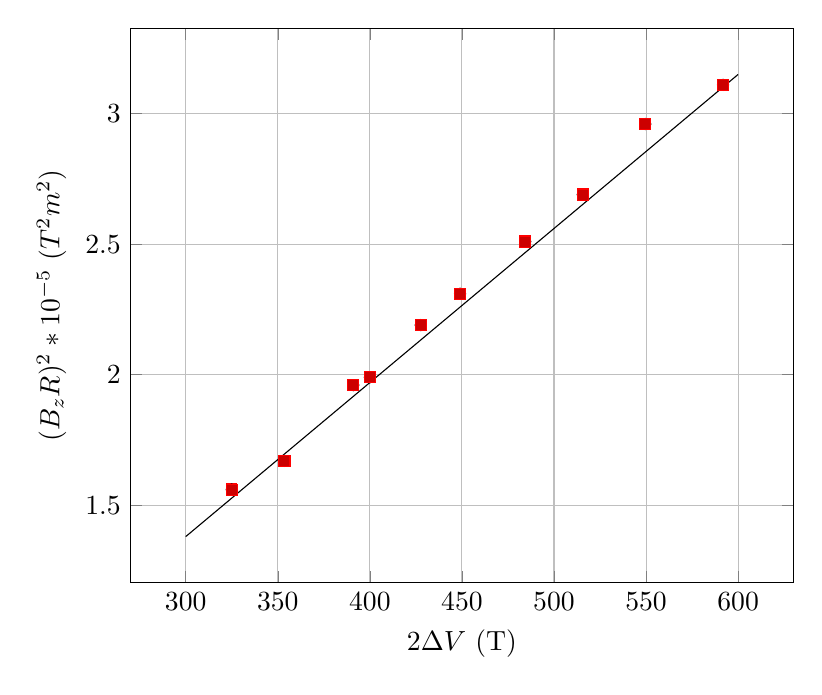
\begin{tikzpicture}
        \begin{axis}
        [
            xlabel={$2\Delta V$ (T)},
            ylabel={$(B_zR)^2*10^{-5}$ ($T^2m^2$)},
            grid=both,
            scatter/classes={
                a={mark=o,draw=black},
                b={mark=o,draw=black,fill=black}
            }
        ]
        \addplot[scatter,only marks,scatter src=explicit symbolic] 
            table[meta=label] {
              x     y    xerror yerror    label
            325     1.56   0.1     0.022      b
            353.6	1.67   0.1     0.014      a
            391	    1.96   0.1     0.014      a
            427.6	2.19   0.1     0.014      a
            449     2.31   0.1     0.014      a
            484.4   2.51   0.1       0        a
            515.6   2.69   0.1       0        a  
            549.6   2.96   0.1       0        a
            591.8   3.11   0.1       0        a
            400     1.99   0.1       0        a
         
        };
        \addplot+[
            only marks,
            error bars/.cd,
            x dir=both, x explicit,
            y dir=both, y explicit
        ] table[x=x, y=y, x error=xerror, y error=yerror] {
                x     y    xerror yerror    label
            325     1.56   0.1     0.022      b
            353.6	1.67   0.1     0.014      a
            391	    1.96   0.1     0.014      a
            427.6	2.19   0.1     0.014      a
            449     2.31   0.1     0.014      a
            484.4   2.51   0.1       0        a
            515.6   2.69   0.1       0        a  
            549.6   2.96   0.1       0        a
            591.8   3.11   0.1       0        a
            400     1.99   0.1       0        a
        };
        \addplot[
    domain=300:600,
    samples=100,
    color=black
] {0.0059*x - 0.39};
    \end{axis}
    \end{tikzpicture}
    \caption{Linear regression between $(B_zR)^2$ and the voltage for the orthogonal setup. }
\end{figure}

%paralello
\begin{figure}[H]
    \centering
    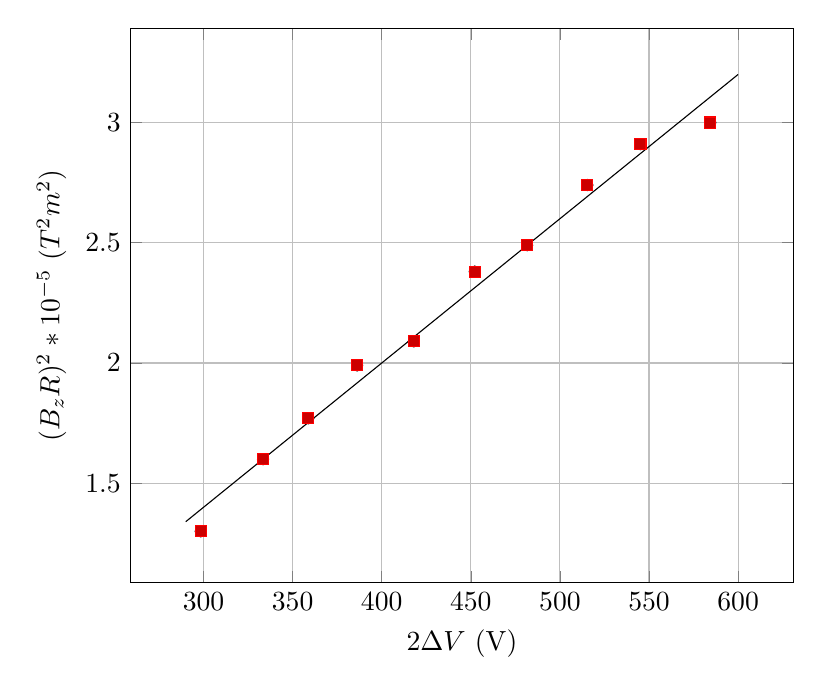
\begin{tikzpicture}
        \begin{axis}
        [
            xlabel={$2\Delta V$ (V)},
            ylabel={$(B_zR)^2*10^{-5}$ ($T^2m^2$)},
            grid=both,
            scatter/classes={
                a={mark=o,draw=black},
                b={mark=o,draw=black,fill=black}
            }
        ]
        \addplot[scatter,only marks,scatter src=explicit symbolic] 
            table[meta=label] {
              x     y    xerror yerror    label
            298.4   1.30   0.1     0.022      b
            333.4	1.60   0.1     0.014      a
            358.8   1.77   0.1     0.014      a
            386.2	1.99   0.1     0.014      a
            418     2.09   0.1     0.014      a
            452.2   2.38   0.1       0        a
            481.6   2.49   0.1       0        a  
            515.4   2.74   0.1       0        a
            545.2   2.91   0.1       0        a
            584.4   3.00   0.1       0        a
         
        };
        \addplot+[
            only marks,
            error bars/.cd,
            x dir=both, x explicit,
            y dir=both, y explicit
        ] table[x=x, y=y, x error=xerror, y error=yerror] {
             x     y    xerror yerror    label
            298.4   1.30   0.1     0.022      b
            333.4	1.60   0.1     0.014      a
            358.8   1.77   0.1     0.014      a
            386.2	1.99   0.1     0.014      a
            418     2.09   0.1     0.014      a
            452.2   2.38   0.1       0        a
            481.6   2.49   0.1       0        a  
            515.4   2.74   0.1       0        a
            545.2   2.91   0.1       0        a
            584.4   3.00   0.1       0        a
        };
        \addplot[
    domain=290:600,
    samples=100,
    color=black
] {0.0060*x - 0.40};
    \end{axis}
    \end{tikzpicture}
    \caption{Linear regression between $(B_zR)^2$ and the voltage for the parallel setup. }
\end{figure}

%antiparallelo

\begin{figure}[H]
    \centering
    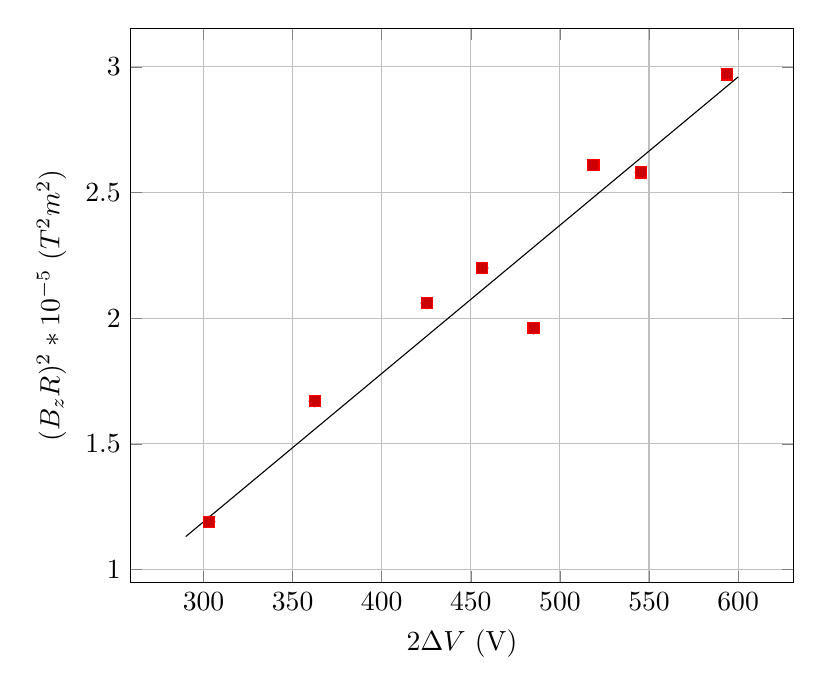
\begin{tikzpicture}
        \begin{axis}
        [
            xlabel={$2\Delta V$ (V)},
            ylabel={$(B_zR)^2*10^{-5}$ ($T^2m^2$)},
            grid=both,
            scatter/classes={
                a={mark=o,draw=black},
                b={mark=o,draw=black,fill=black}
            }
        ]
        \addplot[scatter,only marks,scatter src=explicit symbolic] 
            table[meta=label] {
              x     y    xerror yerror    label
            303.2   1.19   0.1     0.022      b
            362.4	1.67   0.1     0.014      a
            425.2   2.06   0.1     0.014      a
            485.2	1.96   0.1     0.014      a
            545.4   2.58   0.1     0.014      a
            593.8   2.97   0.1       0        a
            518.8   2.61   0.1       0        a  
            456.4   2.20   0.1       0        a
        };
        \addplot+[
            only marks,
            error bars/.cd,
            x dir=both, x explicit,
            y dir=both, y explicit
        ] table[x=x, y=y, x error=xerror, y error=yerror] {
               x     y    xerror yerror    label
            303.2   1.19   0.1     0.022      b
            362.4	1.67   0.1     0.014      a
            425.2   2.06   0.1     0.014      a
            485.2	1.96   0.1     0.014      a
            545.4   2.58   0.1     0.014      a
            593.8   2.97   0.1       0        a
            518.8   2.61   0.1       0        a  
            456.4   2.20   0.1       0        a
        };
        \addplot[
    domain=290:600,
    samples=100,
    color=black
] {0.0059*x - 0.58};
    \end{axis}
    \end{tikzpicture}
    \caption{Linear regression between $(B_zR)^2$ and the voltage for the antiparallel setup.}
\end{figure}
The final values were found to be:
\begin{align*}
    &\frac{e}{m}=(1.67\pm0.01)\, \mathrm{C/Kg}\,\, (Orthogonal)\\
    &\frac{e}{m}=(1.66\pm0.01)\, \mathrm{C/Kg}\,\, (Parallel)\\
    &\frac{e}{m}=(1.68\pm0.01)\, \mathrm{C/Kg}\,\, (Antiparallel)\\
\end{align*}
which doesn't correlates with the accepted value of:
\begin{equation*}
    \frac{e}{m}=1.76\,\,\, \mathrm{C/Kg}
\end{equation*}

%Confronto con i dati noti e valutazione di discrepanze.
\section{Conclusion}
test

\end{document}

